\documentclass[12pt]{article}
\usepackage{amsmath}
\usepackage{array}
% \usepackage{gensymb}
\usepackage{geometry}
\usepackage{graphicx}
\usepackage{pgfplots}
\usepackage{siunitx}
\usepackage{wrapfig}

\title{Homework \#12}
\author{Donald Aingworth IV}
\date{November 13, 2024}

\pgfplotsset{width=8cm,compat=1.9}
\usepgfplotslibrary{external}
% \tikzexternalize

\begin{document}

\DeclareSIUnit{\mile}{mi}
\DeclareSIUnit{\gal}{gal}
\DeclareSIUnit{\foot}{ft}
\DeclareSIUnit{\h}{h}

\maketitle

\pagebreak

\section*{Problem 1}
In 1932, James Chadwick fired neutrons of unknown speed and mass into different
substances. He found that protons (of mass 1 u) were given a speed 7.5 times that given to
nitrogen nuclei (of mass 14 u). If the collisions were elastic and head on, what can you deduce
about the mass of the neutron?

\subsection*{Solution}


\pagebreak
\section*{Problem 2}
A one-dimensional inelastic collision may be characterized by a coefficient of restitution $e$ that relates the relative velocities before and after the collision: $(v_{1,f} - v_{2,f}) = -e(v_{1,i} i v{2,i})$. Show that the final velocities are:
\[ v_{1,f} = \frac{(m_1 - em_2)v_{1,i} + m_2(1 + e)v_{2,i}}{m_1 + m_2} \]
\[ v_{2,f} = \frac{m_1(1 + e)v_{1,i} + (m_2 - em_1)v_{2,i}}{m_1 + m_2} \]

\textit{(Hint, kinetic energy is not conserved. You will need two equations so solve for the two
unknowns.)}
\subsection*{Solution}


\pagebreak
\section*{Problem 3}
An alpha particle ($^4$He) undergoes an elastic collision with a stationary uranium nucleus ($^{235}$U). What
percent of the kinetic energy of the alpha particle is transferred to the uranium nucleus? Assume the
collision is one dimensional.

\subsection*{Solution}


\pagebreak
\section*{Problem 4}
\begin{wrapfigure}{r}{0.35\textwidth}
    \vspace{-30pt}
    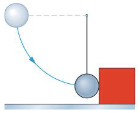
\includegraphics[width=0.35\textwidth]{graph_4.png} 
    % \label{fig:wrapfig}
\end{wrapfigure}
A steel ball of mass 0.500 kg is fastened to a cord that is 70.0 cm long and fixed at the far end. The
ball is then released when the cord is horizontal. At the bottom of its path, the ball strikes a 2.50 kg steel
block initially at rest on a frictionless surface. The collision is elastic. Find (a) the speed of the ball and
(b) the speed of the block, both just after the collision.

\subsection*{Solution}


\pagebreak
\section*{Problem 5}
The platter in a belt drive turntable is driven by a belt that wraps around a hub, of radius 3.00
cm, below the platter and around the shaft of the motor. If the platter rotates at 33.3 rpm and the
motor rotates at 60 rpm, what is the required radius of the shaft?

\subsection*{Solution}


\pagebreak
\section*{Problem 6}
At t = 0, a flywheel has an angular velocity of 4.70 rad/s, a constant angular acceleration of
-0.24 rad/s$^2$, and a reference line at $\theta_0 = 0$. (a) Through what maximum angle $\theta_{max}$ will the
reference line turn in the positive direction? What are the (b) first and (c) second times the reference line will be at $\theta = \frac{1}{2}\theta_{max}$? At what (d) negative time and (e) positive time will the
reference line be at $\theta$ = -10.5 rad? (f) Graph $\theta$ versus t, and indicate your answers.

\subsection*{Solution}


\pagebreak
\section*{Problem 7}
\begin{wrapfigure}{r}{0.35\textwidth}
    \vspace{-30pt}
    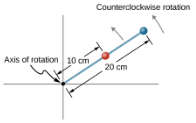
\includegraphics[width=0.35\textwidth]{graph_7.png} 
    % \label{fig:wrapfig}
\end{wrapfigure}
The angular position of a rod varies as 20.0 $t^2$ radians starting from time t = 0 . The rod has
two beads on it as shown in the following figure, one at 10.0 cm from the rotation axis and the
other at 20.0 cm from the rotation axis. (a) What is the instantaneous angular velocity of the rod
at t = 5.00 s? (b) What is the angular acceleration of the rod? (c) What are the tangential speeds
of the beads at t = 5.00 s? (d) What are the tangential accelerations of the beads at t = 5.00 s? (e)
What are the centripetal accelerations of the beads at t = 5.00 s?

\subsection*{Solution}


\pagebreak
\section*{Problem 8}
The angular acceleration of a rotating rigid body is given by $\alpha = (A - Bt)$, where A =
2.00 rad/s$^2$ and B = 3.00 rad. If the body starts rotating from rest at t = 0 , (a) what is the angular
velocity? (b) Angular position? (c) What angle does it rotate through in 10.0 s? (d) Where does
the vector perpendicular to the axis of rotation indicating 0\unit{\degree} at t = 0 lie at t = 10.0 s ?

\subsection*{Solution}
\subsubsection*{Section (a)}
We remark that since $\alpha = \frac{d\omega}{dt}$, we can manipulate it to know that $\omega = \int \alpha\ dt$. We also know that $\omega = 0$ at $t = 0$.
\begin{align*}
    \alpha  &=  A - Bt\\
    \omega  &=  \int \alpha\ dt
            =   \int_{0}^{t} A - Bt'\ dt'
            =   \left[At' - \frac{Bt'^2}{2}\right]_0^t\\
            &=  At - \frac{1}{2}Bt^2
            =   \boxed{2.00t - \frac{3}{2}t^2}
\end{align*}

\subsubsection*{Section (b)}
We remark that since $\omega = \frac{d\theta}{dt}$, we can manipulate it to know that $\theta = \int \omega\ dt$. We also assume that $\theta = 0$ at $t = 0$.
\begin{align*}
    \alpha  &=  A - Bt\\
    \omega  &=  At - \frac{1}{2}Bt^2\\
    \theta  &=  \int \omega\ dt
            =   \int_{0}^{t} At' - \frac{1}{2}Bt'^2\ dt'
            =   \left[\frac{At'^2}{2} - \frac{Bt'^3}{6}\right]_0^t\\
            &=  \frac{At^2}{2} - \frac{Bt^3}{6}
            =   \boxed{t^2 - \frac{1}{2}t^3}
\end{align*}

% \pagebreak
\subsubsection*{Section (c)}


\end{document}